\chapter{Exigências Específicas}
	O sistema deve ser implementado contendo as funcionalidades referentes aos tópicos apresentados abaixo. Cada tópico será avaliado separadamente. Para o aluno obter nota máxima em cada tópico, ele precisa utilizar todas as estruturas listadas nos respectivos sub-tópicos. Também serão consideradas as boas práticas de programação em JavaScript, uso adequado de notações e conceitos aprendidos, organização do código e criatividade.

\section{Qualidade do código}
Estes itens foram retirado conforme combinado em sala de aula.
Style Guide
Strict mode
\subsection{Hint}
	Objetivo: mostrar a correção de apenas 5 problemas informados pelo lint ou hint.
	
Problema 1
\begin{figure}[!htb]
\setcounter{figure}{0}
\centering
\begin{minipage}{.5\textwidth}
  \centering
  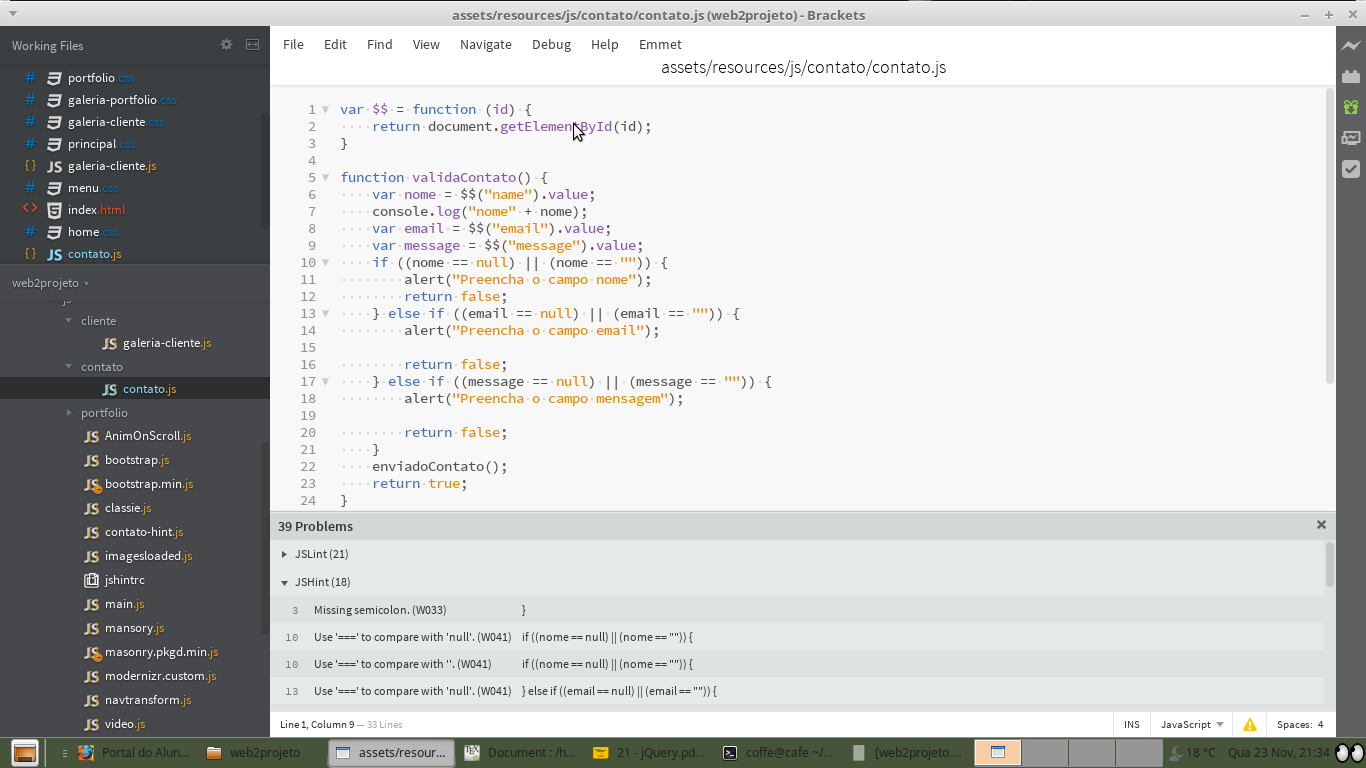
\includegraphics[width=.9\linewidth]{./img/hint1.png}
  \captionof{figure}{Problema 1}
\end{minipage}%
\begin{minipage}{.5\textwidth}
  \centering
  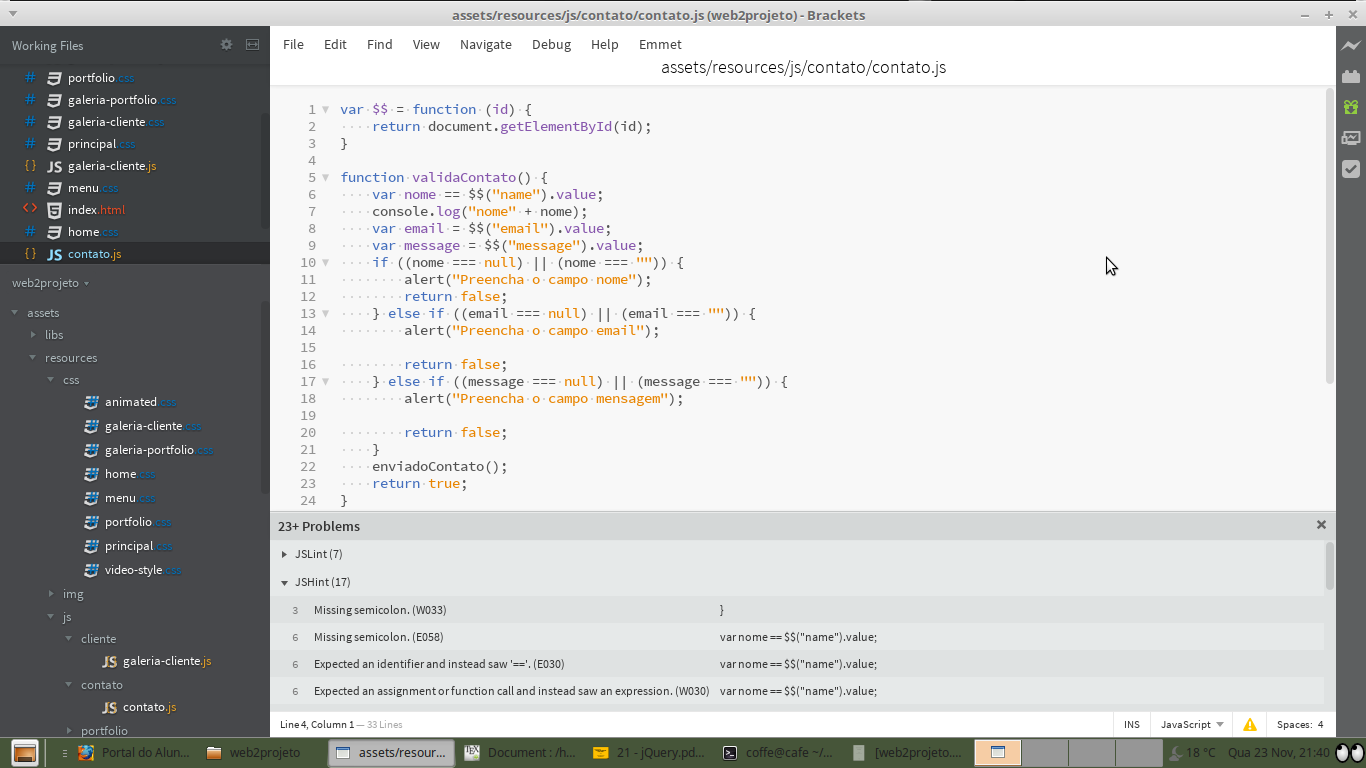
\includegraphics[width=.7\linewidth]{./img/hint1-arrumado.png}
  \captionof{figure}{Problema 1 - Correção}
\end{minipage}
\end{figure}	

Problema 2
\begin{figure}[!htb]
\setcounter{figure}{0}
\centering
\begin{minipage}{.5\textwidth}
  \centering
  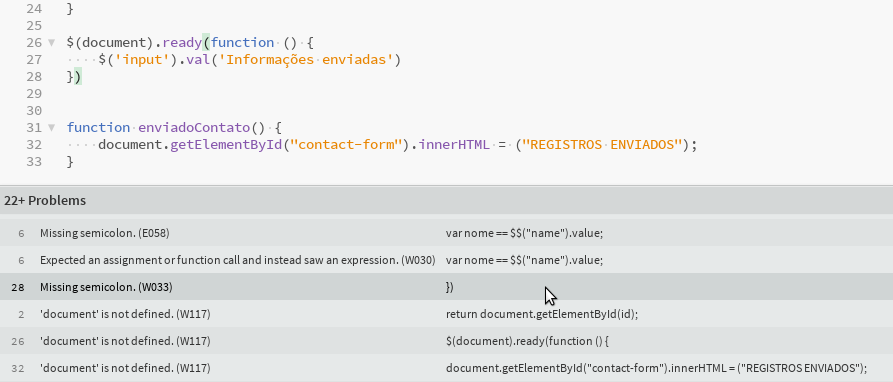
\includegraphics[width=.9\linewidth]{./img/hint2.png}
  \captionof{figure}{Problema 2}
\end{minipage}%
\begin{minipage}{.5\textwidth}
  \centering
  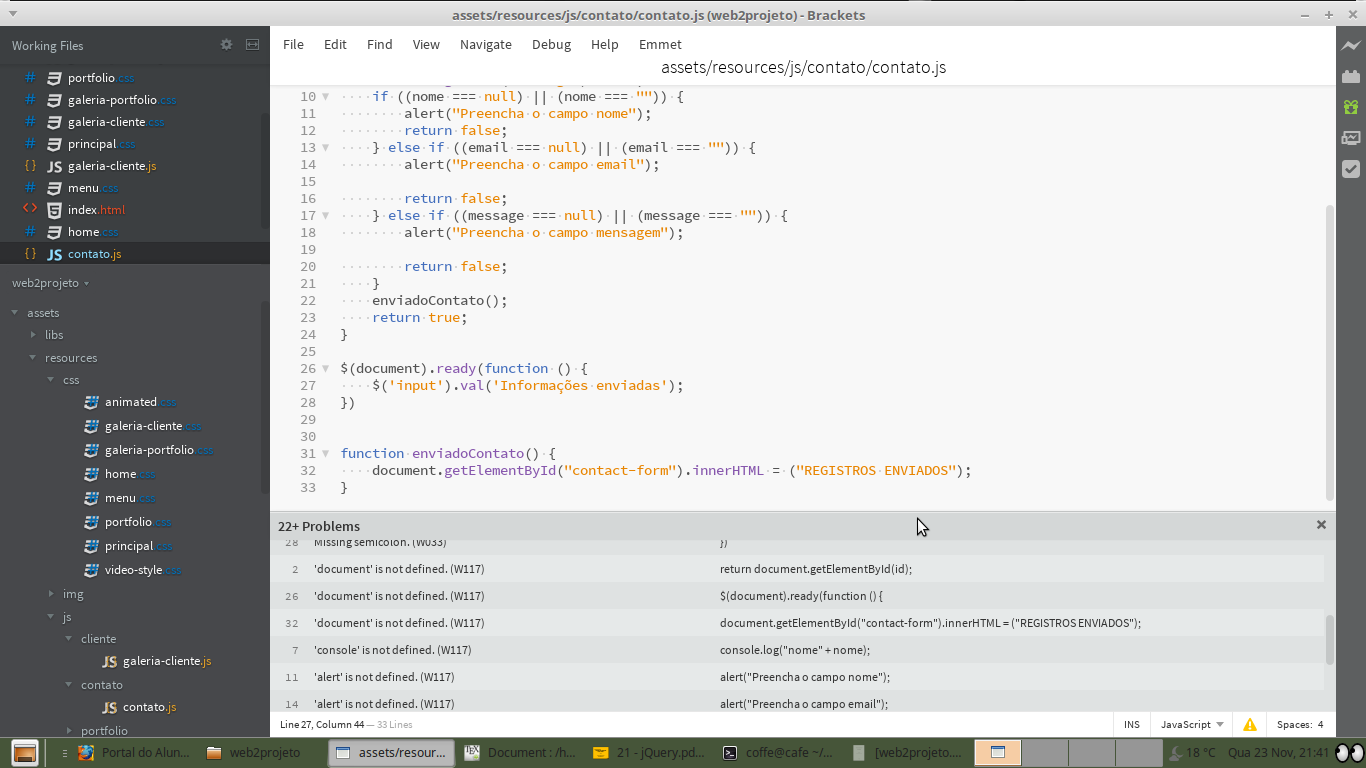
\includegraphics[width=.7\linewidth]{./img/hint2-arrumado.png}
  \captionof{figure}{Problema 2 - Correção}
\end{minipage}
\end{figure}	


Problema 3
\begin{figure}[!htb]
\setcounter{figure}{0}
\centering
\begin{minipage}{.5\textwidth}
  \centering
  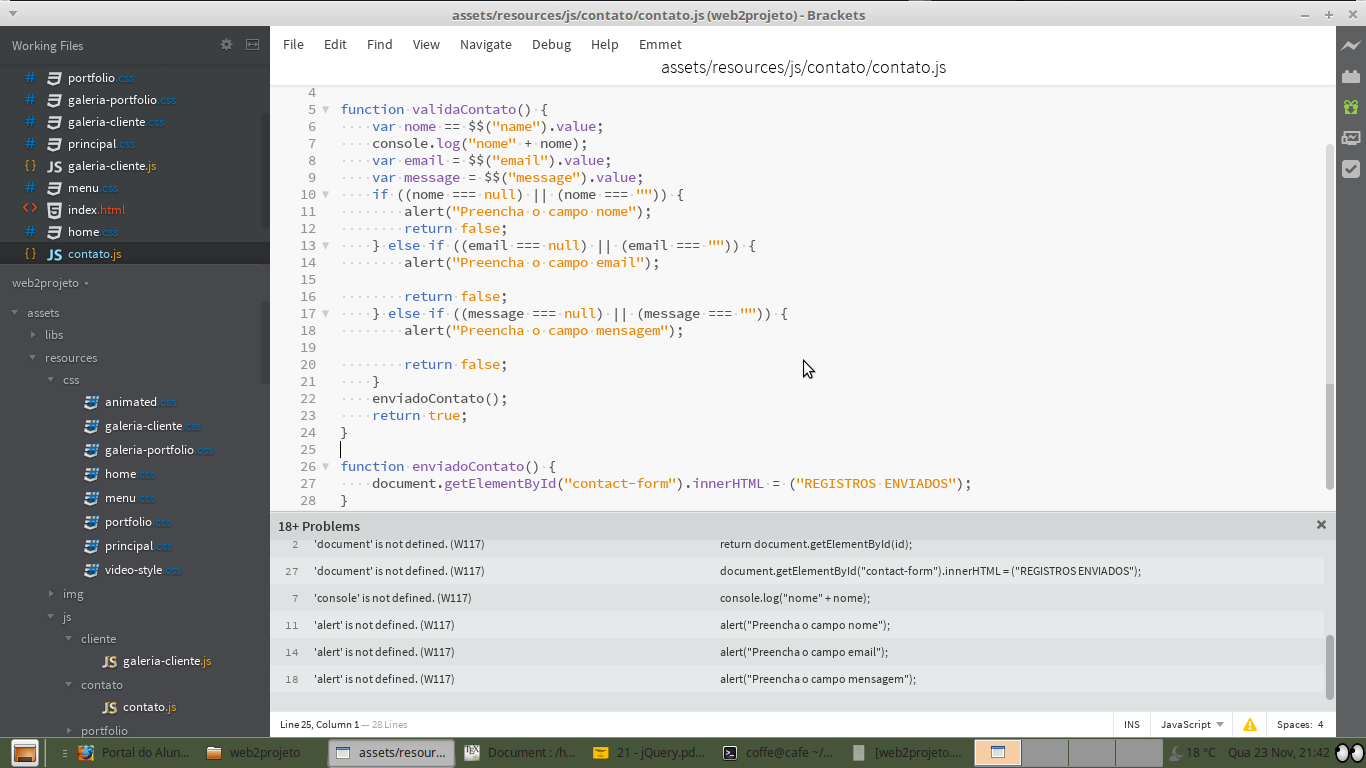
\includegraphics[width=.9\linewidth]{./img/hint3.png}
  \captionof{figure}{Problema 3}
\end{minipage}%
\begin{minipage}{.5\textwidth}
  \centering
  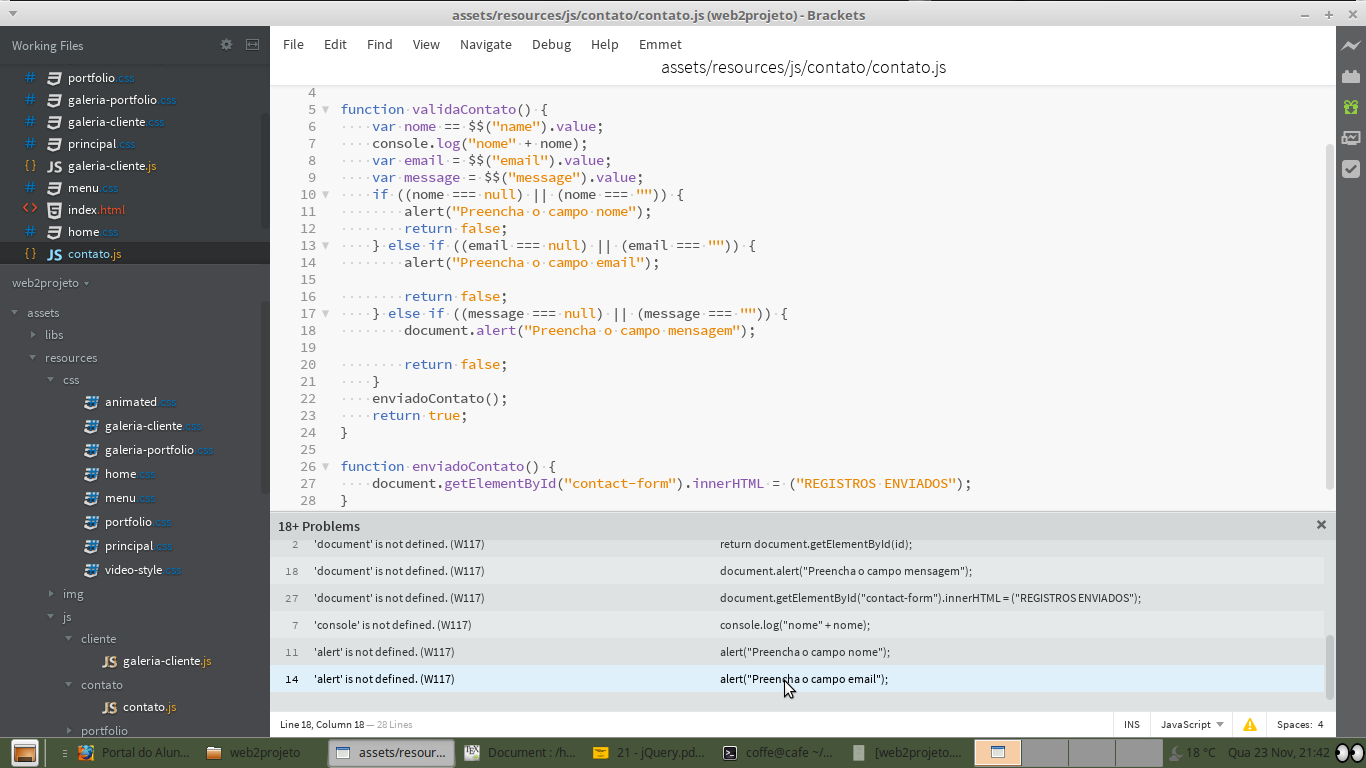
\includegraphics[width=.7\linewidth]{./img/hint3-arrumado.png}
  \captionof{figure}{Problema 3 - Correção}
\end{minipage}
\end{figure}

Problema 4
\begin{figure}[!htb]
\setcounter{figure}{0}
\centering
\begin{minipage}{.5\textwidth}
  \centering
  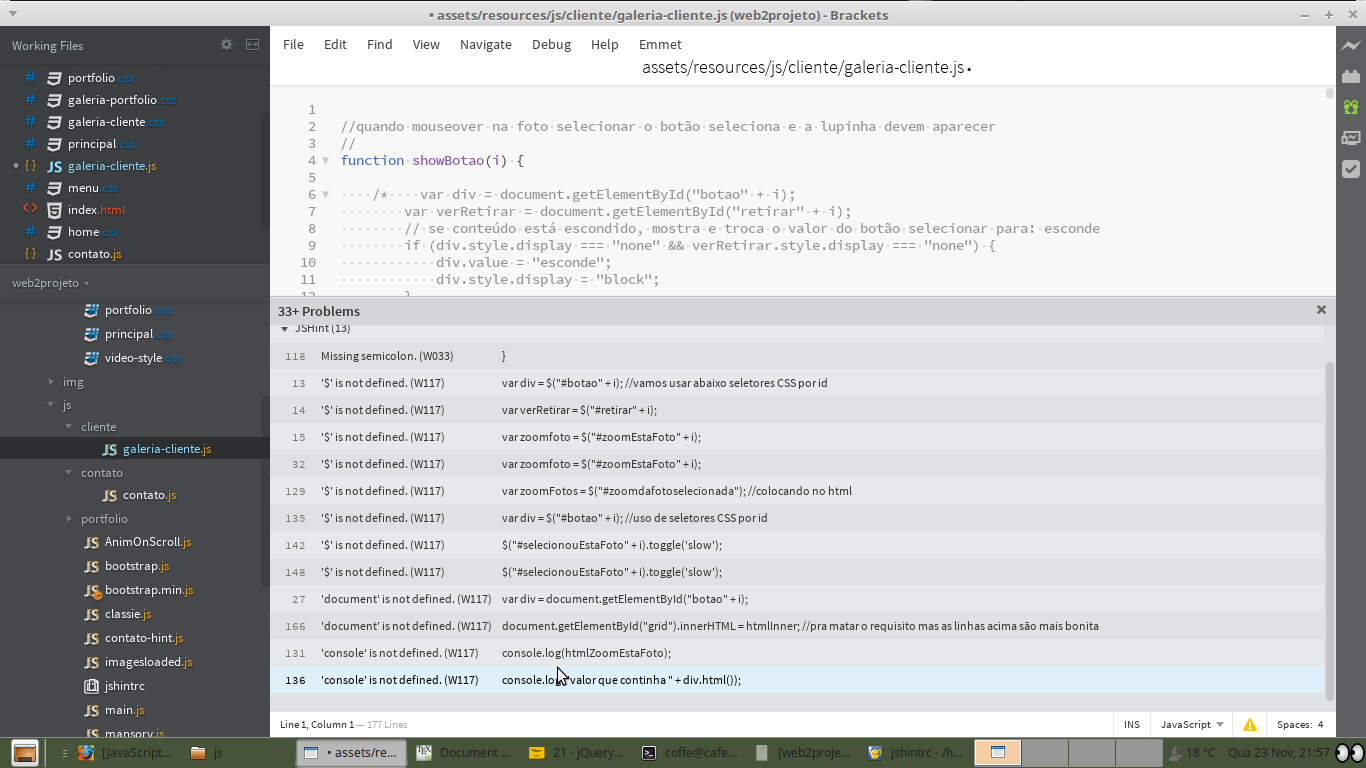
\includegraphics[width=.9\linewidth]{./img/hint4.png}
  \captionof{figure}{Problema 4}
\end{minipage}%
\begin{minipage}{.5\textwidth}
  \centering
  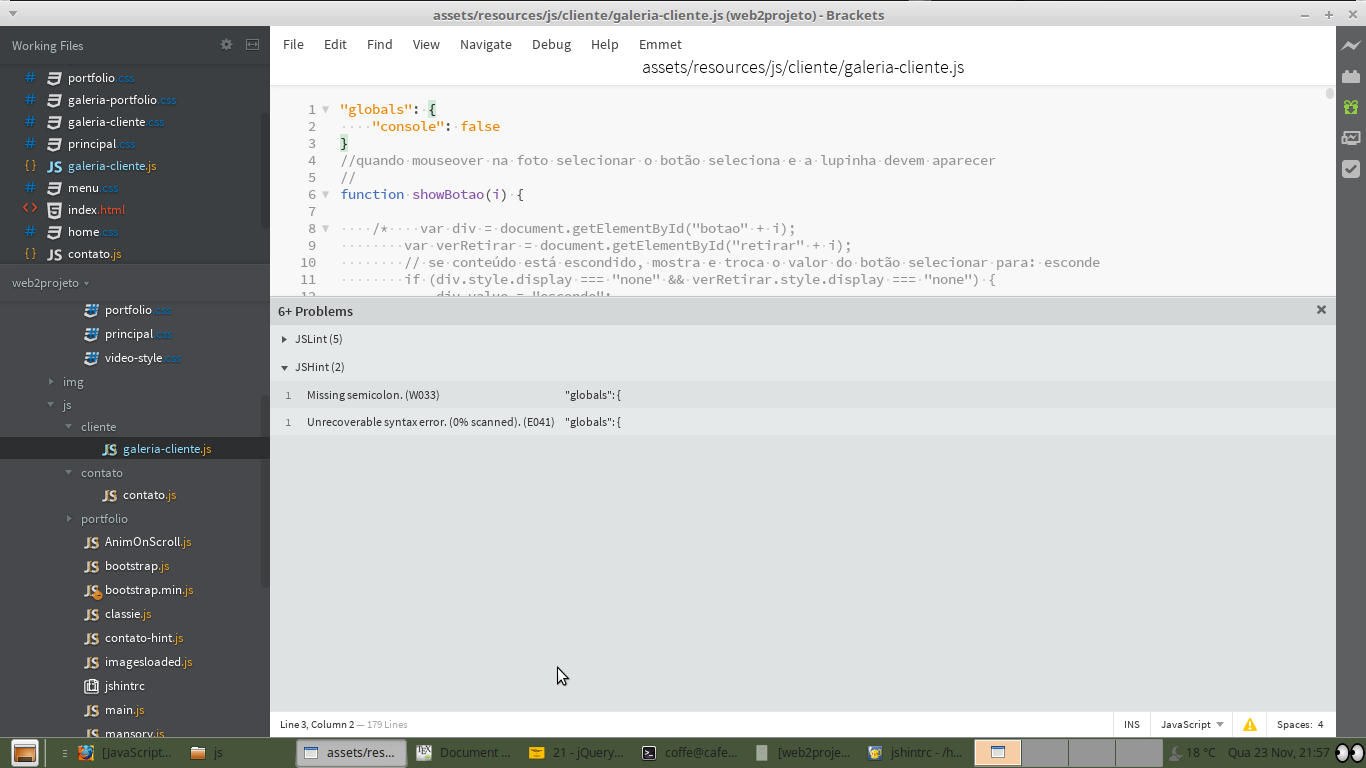
\includegraphics[width=.7\linewidth]{./img/hint4-arrumado.png}
  \captionof{figure}{Problema 4 - Correção}
\end{minipage}
\end{figure}	

\section{Caixas de Diálogo}

\subsection{prompt}

\subsection{alert}

	No arquivo $JavaScript$ chamado $contato.js$ criamos uma função com nome $validaContato()$ conforme segue abaixo para melhor visualização:
\begin{lstlisting}
function validaContato() {
    var nome = $$("name").value;
    console.log("nome" + nome);
    var email = $$("email").value;
    var message = $$("message").value;
    if ((nome == null) || (nome == "")) {
        alert("Preencha o campo nome");
        return false;
    } else if ((email == null) || (email == "")) {
        alert("Preencha o campo email");
        return false;
    } else if ((message == null) || (message == "")) {
        alert("Preencha o campo mensagem");
        return false;
    }
    return true;
}
\end{lstlisting}
	Esta função está relacionada a validação dos campos do formulário. E dentro dela utilizamos $alert$ para enviar uma mensagem ao visitante da página.

\subsection{confirm}

\section{Funções}
\subsection{Função anônima com argumento}

\subsection{Função anônima sem argumento}

\subsection{Função anônima auto-executável}

\subsection{Função com nome}

	No arquivo $JavaScript$ chamado $contato.js$ criamos uma função com nome $validaContato()$ conforme segue abaixo para melhor visualização:
\begin{lstlisting}
function validaContato() {
    var nome = $$("name").value;
    console.log("nome" + nome);
    var email = $$("email").value;
    var message = $$("message").value;
    if ((nome == null) || (nome == "")) {
        alert("Preencha o campo nome");
        return false;
    } else if ((email == null) || (email == "")) {
        alert("Preencha o campo email");
        return false;
    } else if ((message == null) || (message == "")) {
        alert("Preencha o campo mensagem");
        return false;
    }
    return true;
}
\end{lstlisting}
	Esta função está relacionada a validação dos campos do formulário.

\subsection{Função aninhada/interna}

\subsection{Passagem de uma função como parâmetro}

\section{Eventos}

\subsection{Evento de carregamento do documento}


\subsection{Evento de movimento do mouse}


\subsection{Evento de teclado}
 Objetivo:  - usar charCode ou KeyCode.
 
 
\subsection{Eventos de formulário}
Objetivo: onfocus e onblur.


\subsection{objeto event}
Obejtivo: Imprimir alguma propriedade do objeto event recebido como parâmetro

\subsection{Propagação de eventos no modelo bolha}

\section{Acesso aos elementos DOM do HTML }

\subsection{Via acesso direto}

 Pelo id do elemento HTML
 
\subsection{Via getElementByID()}
	Ver arquivo $contato.html$ a função $enviadoContato()$, conforme código abaixo:
	
\begin{lstlisting}
function enviadoContato() {
    document.getElementById("contact-form").innerHTML = ("REGISTROS ENVIADOS");
}
\end{lstlisting}

\subsection{Via getElementsByName()}



\subsection{Via getElementsByTagName()}



\subsection{Via seletores CSS}
  Usados na função querySelector() ou jQuery
  
\section{Tratadores de Evento}
\subsection{Evento inline}
Objetivo: especificar o tratador de evento inline

tratador de eventos inline - onmouseover, onmouseout, onclick

$onclick$ - Ver no arquivo $galeria-cliente.js$ a seguinte linha:

\begin{lstlisting}
<button id="botao' + i + '" style="display:none" class="btn btn-success" onclick="alternarEscolhaDaFoto(' + i + ');">Selecionar</button>
\end{lstlisting}

	Esta linha irá criar o botão Selecionar. Nela é mostrado uma ação para $onclick$ que chama a função $alternarEscolhaDaFoto(i)$ - I $i$ é um parâmetro referente a foto que estará sendo mostrada.

\subsection{Modo tradicional}
Objetivo: especificar o tratador de evento no carregamento da página HTML no modo tradicional.


\subsection{addEventListener}
 Objetivo: especificar o tratador de evento no carregamento da página HTML com a função addEventListener.
 
\subsection{Operador this}
 Objetivo: usar o operador this em funções tratadoras de eventos.
 
 


\section{Formulário}
	Foi criado a página $contato.html$. Nesta página temos um formulário com $3$ campos de preenchimento obrigatórios.
	
\subsection{Validação}
	Objetivo: validação de formulário com onsubmit usando os métodos tradicionais.
	
	Para cumprir o objetivo o formulário $contato.html$ faz uso da seguinte maneira:
\begin{lstlisting}
<form id="contact-form" class="validate-form" method="post" onsubmit="return validaContato()">
\end{lstlisting}

	O arquivo $JavaScript$ chamado $contato.js$ contém a função com nome $validaContato()$:
\begin{lstlisting}
function validaContato() {
    var nome = $$("name").value;
    console.log("nome" + nome);
    var email = $$("email").value;
    var message = $$("message").value;
    if ((nome == null) || (nome == "")) {
        alert("Preencha o campo nome");
        return false;
    } else if ((email == null) || (email == "")) {
        alert("Preencha o campo email");

        return false;
    } else if ((message == null) || (message == "")) {
        alert("Preencha o campo mensagem");

        return false;
    }
    enviadoContato();
    return true;
}
\end{lstlisting}
	

\subsection{Propriedade Value}
	Objetivo: ler e escrever em elementos $input$ com a propriedade $value$
	
\begin{lstlisting}
$(document).ready(function () {
    $('input').val('Informacoes enviadas')
})
\end{lstlisting}


\subsection{innerHtml}
	Objetivo: alterar o conteúdo de elementos $div$ ou $p$com a propriedade $innerHTML$
	
	Para este item escolhemos alterar o elemento $div$ do formulário de $contatos$ pois assim que o visitante enviar uma mensagem de contato a estrutura do formulário será substituída por uma frase, conforme código abaixo, definido pela função.

\begin{lstlisting}
function enviadoContato() {
    document.getElementById("contact-form").innerHTML = ("REGISTROS ENVIADOS");
}
\end{lstlisting}


\subsection{checkbox, radio ou select}
Manipulação de elemento de listagem, como checkbox, radio ou select


\subsection{Acesso via hierarquia}
Acesso aos elementos de um formulário via hierarquia (caminho) de objetos, ou seja, array forms e elements



\section{Objetos Nativos }
\subsection{Manipulação de array}
Usar métodos para manipulação de array
\subsection{Manipulação de string}
Usar métodos para manipulação de string

\section{Objetos Nativos}
\subsection{Manipulação de array}
Usar métodos para manipulação de array

jsonClienteX na funcao alternarEscolhaDaFoto no arquivo cliente.html



\subsection{Manipulação de string}


Usar métodos para manipulação de string


\section{Objetos}
\subsection{Criar objeto}
Criar objeto usando função construtora ou notação literal


\subsection{Herança}
Usar herança prototipal


\section{jQuery}
\subsection{Seletores CSS}
Uso de seletores CSS - id, classe e tag
\subsection{ID}
	Observa abaixo que na linha 2 do arquivo $galeria-cliente.js$ temos o uso de seletor $CSS$ por $id$.
	
\begin{lstlisting}
function alternarEscolhaDaFoto(i) {
    var div = $("#botao" + i);
    console.log("valor que continha " + div.html());
    if (div.html() == "Selecionar") {
        div.toggle('slow').toggle('slow');
        div.html("Retirar");
        jsonClienteX.fotos[i].escolhido = true;
        div.removeClass('btn-success').addClass('btn-warning');
        $("#selecionouEstaFoto" + i).toggle('slow');
        div.fadeOut(500);
    } else {
        div.html("Selecionar");
        jsonClienteX.fotos[i].escolhido = false;
        div.removeClass('btn-warning').addClass('btn-success');
        $("#selecionouEstaFoto" + i).toggle('slow');
    }
}
\end{lstlisting}
\subsection{classe}


\subsection{tag}



\subsection{Seletores hierarquicos}
Uso de seletores hierarquicos - ancestral/descendente, pai/filho, anterior/proximo
\subsection{Efeitos fade ou slide}

Efeito fadeOut ver cliente.html


\subsection{Tratador de algum evento}
Espeficar o tratador de algum evento via jQuery
\subsection{Manipulação CSS}
	Objetivo: manipulação do CSS via função $css()$ e $addClass()$/$removeClass()$

	Utilizamos $addClass$ e $removeClass$ na função $alternarEscolhaDaFoto(i)$ do arquivo $galeria-cliente.js$. 
	Descrição da função: quando um cliente realizar a seleção de uma foto o botão irá mudar de cor, ficando disponível a opção para desmarcar a foto que acabou de ser selecionada, na função, veja a linha $8$. O inverso irá acontecer quando o cliente desmarcar a foto que havia sido selecionada, linha $13$.
	

\begin{lstlisting}
function alternarEscolhaDaFoto(i) {
    var div = $("#botao" + i);
    console.log("valor que continha " + div.html());
    if (div.html() == "Selecionar") {
        div.toggle('slow').toggle('slow');
        div.html("Retirar");
        jsonClienteX.fotos[i].escolhido = true;
        div.removeClass('btn-success').addClass('btn-warning');
        $("#selecionouEstaFoto" + i).toggle('slow');
        div.fadeOut(500);
    } else {
        div.html("Selecionar");
        jsonClienteX.fotos[i].escolhido = false;
        div.removeClass('btn-warning').addClass('btn-success');
        $("#selecionouEstaFoto" + i).toggle('slow');
    }
}
\end{lstlisting}

\subsection{Manipulação do conteúdo}
	Objetivo: manipulação do conteúdo de um $input$ e $div$ usando $jQuery$.

\section{Web Storage }
\subsection{LocalStorage e SessionStorage}
\subsection{Leitura e escrita de dados simples}
\subsection{Leitura e escrita de JSON}
